\documentclass{article}

\usepackage{fullpage}
\usepackage{amsmath}
\usepackage{amsfonts}
\usepackage{graphicx}
\usepackage{algorithmic}
\usepackage{xcolor}
\usepackage{framed}

\definecolor{dark_red}{rgb}{0.5,0.0,0.0}

\newcommand{\abs}[1]{\left|#1\right|}
\newcommand{\rowvec}[3]{\left\langle #1, #2, #3 \right\rangle}
\newcommand{\colvec}[3]{\begin{bmatrix} #1 \\ #2 \\ #3 \end{bmatrix}}
\newcommand{\at}[1]{\left. #1 \right|}
\newcommand{\diff}[2]{\frac{d #1}{d #2}}
\newcommand{\partdiff}[2]{\frac{\partial #1}{\partial #2}}
\newcommand{\mvec}[1]{\overrightarrow{\mathbf{#1}}}
\newcommand{\pvec}[1]{\overrightarrow{#1}}
\newcommand{\dr}[1]{\textcolor{dark_red}{#1}}



\title{Multi-variable Functions}
\date{}

\begin{document}

\maketitle

\section*{Question 1:}

Draw the domains of the following multi-variable functions. For curves, use solid lines to include the curve as part of the domain, and use dashed lines to exclude the curve from the domain.

\begin{itemize}
\item \(f(x,y) = \frac{\sqrt{-x^2 + 4x}}{\sqrt{9 - x^2 - y^2}}\)
\item \(f(x,y) = \ln(x + y - x^2)\)
\item \(f(x,y) = \frac{\ln(x)}{xy + 2x - 3y - 6}\)
\end{itemize}



\section*{Question 2:}

Compute the following limits:

\begin{itemize}
\item \(\lim_{t \to -1} \colvec{\sqrt{t + 3}}{\frac{t^2}{t+2}}{\ln(t + 5)}\)
\item \(\lim_{(x,y) \to (-1,-2)} \frac{\sqrt{x+y+5}}{x+y+4}\)
\end{itemize}



\section*{Question 3:}

Define the two-variable function \(f(x,y) = \frac{xy}{x^2 + y^2}\).

\subsection*{part 3a:}

Compute the following partial derivatives:
\[\frac{\partial f}{\partial x} \quad \frac{\partial f}{\partial y} \quad \frac{\partial^2 f}{\partial x^2} \quad \frac{\partial^2 f}{\partial y^2} \quad \frac{\partial^2 f}{\partial y \partial x}\] 

\subsection*{part 3b:}

Compute the gradient \(\nabla f\) at the point \((x_0,y_0) = (3,1)\). Compute the equation of the tangent plane to the surface \(z = f(x,y)\) that passes through the point \((x_0,y_0,f(x_0,y_0))\). Given a direction of \(\mathbf{v} = \langle 3, -4 \rangle\), what is the ``directional derivative" of \(f(x,y)\) at \((x_0, y_0)\) in the direction of \(\mathbf{v}\)?



\section*{Question 4:}

\begin{center}
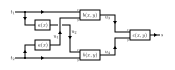
\includegraphics[width = \textwidth]{chain_rule_XOR_circuit}
\end{center}

In the flow-chart (arithmetic circuit) above, the output quantity \(s\) is being computed from input quantities \(t_1\) and \(t_2\). There are the internal variables \(u_1\), \(u_2\), \(u_3\), and \(u_4\).

\subsection*{part 4a:}

Build expressions for \(u_1\), \(u_2\), \(u_3\), \(u_4\), and \(s\) from the input parameters \(t_1\) and \(t_2\), and the functions \(a(x)\), \(b(x,y)\), and \(c(x,y)\).

\subsection*{part 4b:}

Without any knowledge of \(a(x)\), \(b(x,y)\), or \(c(x,y)\), derive expressions for the following partial derivatives: \(\partdiff{u_1}{t_1}\), \(\partdiff{u_1}{t_2}\), \(\partdiff{u_2}{t_1}\), and \(\partdiff{u_2}{t_2}\).

Derive expressions for the following partial derivatives: \(\partdiff{u_3}{t_1}\), \(\partdiff{u_3}{t_2}\), \(\partdiff{u_4}{t_1}\), and \(\partdiff{u_4}{t_2}\) in terms of the partial derivatives computed previously.

Derive expressions for the following partial derivatives: \(\partdiff{s}{t_1}\), and \(\partdiff{s}{t_2}\) in terms of the partial derivatives computed previously.

\subsection*{part 4c:}

Now let \(a(x) = 1 - x\), \(b(x,y) = xy\), and \(c(x,y) = x + y - xy\). Compute all first-order derivatives: \(\frac{da}{dx}\), \(\frac{\partial b}{\partial x}\), \(\frac{\partial b}{\partial y}\), \(\frac{\partial c}{\partial x}\), and \(\frac{\partial c}{\partial y}\).

\subsection*{part 4d:}

From the results of the previous sections, compute at \((t_1, t_2) = (3/4, 1/4)\) the output \(s\), as well as the partial derivatives \(\frac{\partial s}{\partial t_1}\) and \(\frac{\partial s}{\partial t_2}\).



\section*{Question 5:}

For each of the following two variable functions \(f(x,y)\), find and classify all of the critical points:

\begin{itemize}
\item \(f(x,y) = -11x^2 + 6xy - 19y^2 + 78x - 94y - 211\)
\item \(f(x,y) = \frac{1}{3}x^3 - \frac{7}{18}x^2 - \frac{2}{3}xy + y^2 - \frac{10}{9}x - \frac{8}{3}y + \frac{16}{9}\)
\item \(f(x,y) = \frac{1}{3}x^3 + \frac{7}{16}x^2 - \frac{3}{2}xy - y^2 - \frac{3}{8}x + \frac{7}{2}y - \frac{49}{16}\)
\item \(f(x,y) = \frac{1}{3}y^3 - x^2 - \frac{3}{2}xy + \frac{7}{16}y^2 - \frac{5}{2}x - \frac{39}{8}y - \frac{25}{16}\)
\item \(f(x,y) = \frac{5}{4}x^4 - \frac{1}{3}x^3 - 2x^2y - 2x^2 + y^2 + 4x\)
\end{itemize}





\end{document}









